% generated by Plantuml 1.2025.4       
\definecolor{plantucolor0000}{RGB}{255,255,255}
\definecolor{plantucolor0001}{RGB}{0,0,0}
\definecolor{plantucolor0002}{RGB}{194,194,194}
\definecolor{plantucolor0003}{RGB}{24,24,24}
\definecolor{plantucolor0004}{RGB}{84,84,84}
\definecolor{plantucolor0005}{RGB}{166,166,166}
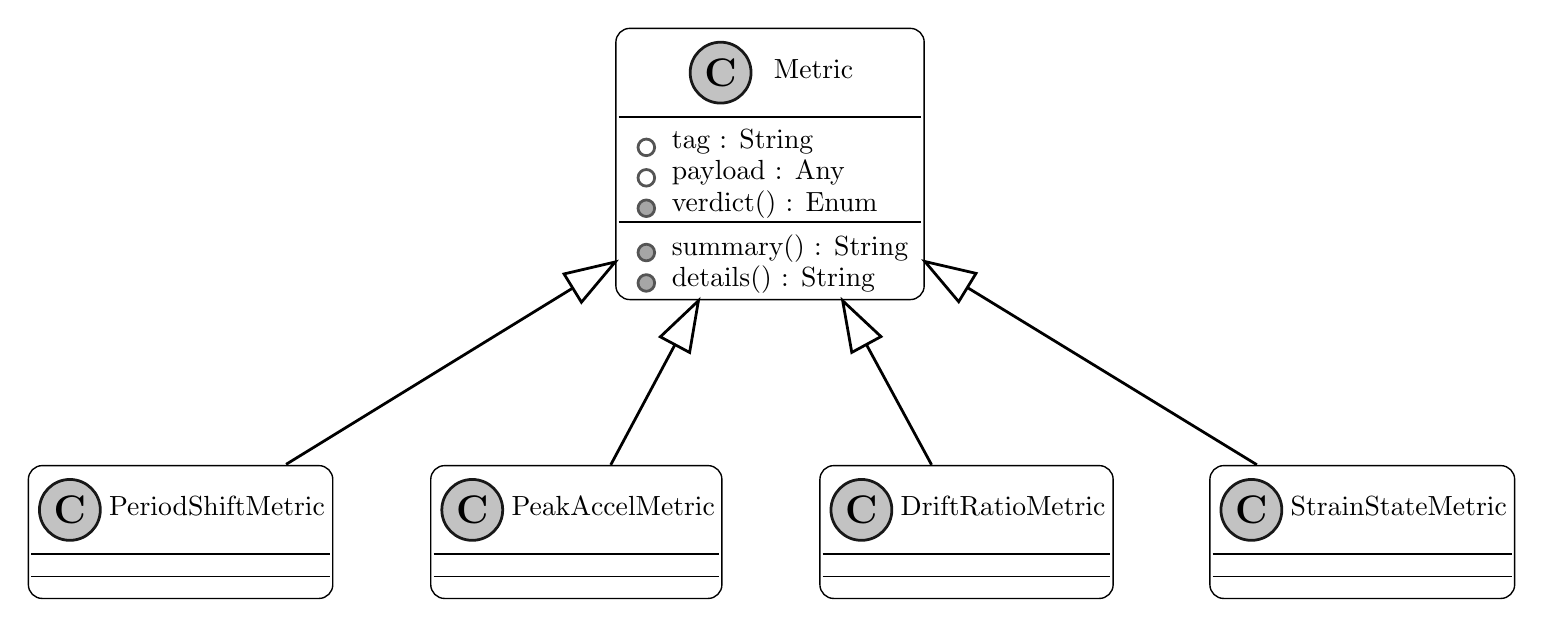
\begin{tikzpicture}[yscale=-1
,pstyle0/.style={color=black,fill=white,line width=0.5pt}
,pstyle1/.style={color=plantucolor0003,fill=plantucolor0002,line width=1.0pt}
,pstyle2/.style={color=black,line width=0.5pt}
,pstyle3/.style={color=plantucolor0004,line width=1.0pt}
,pstyle4/.style={color=plantucolor0004,fill=plantucolor0005,line width=1.0pt}
,pstyle5/.style={color=black,line width=1.0pt}
]
\draw[pstyle0] (219.3pt,12pt) arc (180:270:5pt) -- (224.3pt,7pt) -- (325.7pt,7pt) arc (270:360:5pt) -- (330.7pt,12pt) -- (330.7pt,100pt) arc (0:90:5pt) -- (325.7pt,105pt) -- (224.3pt,105pt) arc (90:180:5pt) -- (219.3pt,100pt) -- cycle;
\draw[pstyle1] (257.142pt,23pt) ellipse (11pt and 11pt);
\node at (257.142pt,23pt)[]{\textbf{\Large C}};
\node at (276.218pt,18pt)[below right,color=black,inner sep=0]{Metric};
\draw[pstyle2] (220.3pt,39pt) -- (329.7pt,39pt);
\draw[pstyle3] (230.3pt,50pt) ellipse (3pt and 3pt);
\node at (239.3pt,43.5pt)[below right,color=black,inner sep=0]{tag : String};
\draw[pstyle3] (230.3pt,61pt) ellipse (3pt and 3pt);
\node at (239.3pt,54.5pt)[below right,color=black,inner sep=0]{payload : Any};
\draw[pstyle4] (230.3pt,72pt) ellipse (3pt and 3pt);
\node at (239.3pt,65.5pt)[below right,color=black,inner sep=0]{verdict() : Enum};
\draw[pstyle5] (220.3pt,77pt) -- (329.7pt,77pt);
\draw[pstyle4] (230.3pt,88pt) ellipse (3pt and 3pt);
\node at (239.3pt,81.5pt)[below right,color=black,inner sep=0]{summary() : String};
\draw[pstyle4] (230.3pt,99pt) ellipse (3pt and 3pt);
\node at (239.3pt,92.5pt)[below right,color=black,inner sep=0]{details() : String};
\draw[pstyle0] (7pt,170pt) arc (180:270:5pt) -- (12pt,165pt) -- (112pt,165pt) arc (270:360:5pt) -- (117pt,170pt) -- (117pt,208pt) arc (0:90:5pt) -- (112pt,213pt) -- (12pt,213pt) arc (90:180:5pt) -- (7pt,208pt) -- cycle;
\draw[pstyle1] (22pt,181pt) ellipse (11pt and 11pt);
\node at (22pt,181pt)[]{\textbf{\Large C}};
\node at (36pt,176pt)[below right,color=black,inner sep=0]{PeriodShiftMetric};
\draw[pstyle2] (8pt,197pt) -- (116pt,197pt);
\draw[pstyle2] (8pt,205pt) -- (116pt,205pt);
\draw[pstyle0] (152.4pt,170pt) arc (180:270:5pt) -- (157.4pt,165pt) -- (252.61pt,165pt) arc (270:360:5pt) -- (257.61pt,170pt) -- (257.61pt,208pt) arc (0:90:5pt) -- (252.61pt,213pt) -- (157.4pt,213pt) arc (90:180:5pt) -- (152.4pt,208pt) -- cycle;
\draw[pstyle1] (167.4pt,181pt) ellipse (11pt and 11pt);
\node at (167.4pt,181pt)[]{\textbf{\Large C}};
\node at (181.4pt,176pt)[below right,color=black,inner sep=0]{PeakAccelMetric};
\draw[pstyle2] (153.4pt,197pt) -- (256.61pt,197pt);
\draw[pstyle2] (153.4pt,205pt) -- (256.61pt,205pt);
\draw[pstyle0] (293.02pt,170pt) arc (180:270:5pt) -- (298.02pt,165pt) -- (393.98pt,165pt) arc (270:360:5pt) -- (398.98pt,170pt) -- (398.98pt,208pt) arc (0:90:5pt) -- (393.98pt,213pt) -- (298.02pt,213pt) arc (90:180:5pt) -- (293.02pt,208pt) -- cycle;
\draw[pstyle1] (308.02pt,181pt) ellipse (11pt and 11pt);
\node at (308.02pt,181pt)[]{\textbf{\Large C}};
\node at (322.02pt,176pt)[below right,color=black,inner sep=0]{DriftRatioMetric};
\draw[pstyle2] (294.02pt,197pt) -- (397.98pt,197pt);
\draw[pstyle2] (294.02pt,205pt) -- (397.98pt,205pt);
\draw[pstyle0] (433.94pt,170pt) arc (180:270:5pt) -- (438.94pt,165pt) -- (539.07pt,165pt) arc (270:360:5pt) -- (544.07pt,170pt) -- (544.07pt,208pt) arc (0:90:5pt) -- (539.07pt,213pt) -- (438.94pt,213pt) arc (90:180:5pt) -- (433.94pt,208pt) -- cycle;
\draw[pstyle1] (448.94pt,181pt) ellipse (11pt and 11pt);
\node at (448.94pt,181pt)[]{\textbf{\Large C}};
\node at (462.94pt,176pt)[below right,color=black,inner sep=0]{StrainStateMetric};
\draw[pstyle2] (434.94pt,197pt) -- (543.07pt,197pt);
\draw[pstyle2] (434.94pt,205pt) -- (543.07pt,205pt);
\draw[pstyle5] (203.7068pt,100.8483pt) ..controls (166.2368pt,123.8883pt) and (133.23pt,144.19pt) .. (100.14pt,164.54pt);
\draw[pstyle5] (219.04pt,91.42pt) -- (200.564pt,95.7372pt) -- (206.8495pt,105.9593pt) -- (219.04pt,91.42pt) -- cycle;
\draw[pstyle5] (240.6505pt,121.2876pt) ..controls (229.8305pt,141.5476pt) and (226.23pt,148.28pt) .. (217.44pt,164.71pt);
\draw[pstyle5] (249.13pt,105.41pt) -- (235.3579pt,118.4611pt) -- (245.943pt,124.1141pt) -- (249.13pt,105.41pt) -- cycle;
\draw[pstyle5] (309.8166pt,121.2353pt) ..controls (320.7966pt,141.4953pt) and (324.47pt,148.28pt) .. (333.38pt,164.71pt);
\draw[pstyle5] (301.24pt,105.41pt) -- (304.5415pt,124.0942pt) -- (315.0917pt,118.3765pt) -- (301.24pt,105.41pt) -- cycle;
\draw[pstyle5] (346.3021pt,100.6474pt) ..controls (384.0721pt,123.7674pt) and (417.58pt,144.28pt) .. (450.91pt,164.68pt);
\draw[pstyle5] (330.95pt,91.25pt) -- (343.1697pt,105.7648pt) -- (349.4346pt,95.5301pt) -- (330.95pt,91.25pt) -- cycle;
\end{tikzpicture}
